The complete-within-a-bound approach of DPOR may not be feasible in large
programs.  We can sacrifice completeness, and instead explore the space of
schedules \emph{randomly}.  We may not find all bugs.  However we still want to
find \emph{most of them}.  Benchmarks show that some scheduling algorithms tend
to be better at this than others; not all algorithms are created equal.  In this
chapter we discuss a number of scheduling algorithms~\sref{algorithms-usual},
propose a new one based on a \emph{weighted} random selection of
threads~\sref{algorithms-swarm}, and show that it performs favourably in a
comparison of standard benchmark programs~\sref{algorithms-eval}.

\section{Concurrency Testing with Randomised Scheduling}
\label{sec:algorithms-usual}

Concurrency testing using randomised scheduling works by repeatedly executing a
concurrent program, exploring a particular schedule on each execution.  Unlike
systematic concurrency testing, little effort is made to avoid repetition of
schedules tested, so these algorithms are incomplete in general.  In this
section we present two approaches to randomised scheduling.

\paragraph{Controlled random scheduling}
A controlled random scheduler uses a random-number generator to choose threads
to execute.  At each scheduling point, a runnable thread is randomly chosen
using a uniform distribution.  This thread is then executed until the next
scheduling point.  Like any controlled scheduling technique, the executed
schedule can be recorded and replayed.  Additionally, a random scheduler can be
used on programs that exhibit nondeterminism beyond scheduler nondeterminism,
although in this case schedule replay will be unreliable\cite{thomson2016}.

\paragraph{Probabilistic concurrency testing}
The PCT algorithm\cite{burckhardt2010} uses a priority-based scheduler where the
highest priority runnable thread is chosen at each scheduling point.  A bounded
number of \emph{priority change points} are inserted in the execution which
change the priority of the currently executing thread to a low value.  These
change points are distributed uniformly over the length of the execution.

The algorithm is described as follows\cite{burckhardt2010}: given a program with
at most $n$ threads and at most $k$ steps, choose a bound $d$, then:

\begin{enumerate}
\item Randomly assign each of the $n$ threads a distinct initial priority value
  from $\{d, d + 1, \ldots, d+n\}$.  The lower priority values
  $\{1, \ldots, d−1\}$ are reserved for change points.
\item Uniformly pick integers $c_1, \ldots, c_{d−1}$ from $\{1, \ldots, k\}$.
  These will be the priority change points.
\item Schedule threads strictly according to their priorities: never schedule a
  thread if a higher priority thread is runnable.  After executing the $c_i$-th
  step $(1 \leq i < d)$, change the priority of the thread that executed the
  step to $i$.
\end{enumerate}

PCT also introduces the idea of a ``bug depth''.  The bug depth is defined as
the minimum set of ordering constraints between actions from different threads
that are sufficient to trigger the bug\cite{burckhardt2010}.  Assuming a bug
with depth $d$, the probability of the PCT algorithm detecting the bug on a
single execution is $1/nk^{d−1}$.

The intuition behind PCT is that many concurrency bugs typically require
orderings between only a few actions to appear.

\section{Weighted Random Scheduling and Swarm Testing}
\label{sec:algorithms-swarm}

We now present \emph{swarm scheduling}, our new algorithm for finding
concurrency bugs through controlled scheduling.  The algorithm is inspired by
\emph{swarm testing}\cite{groce2012}, an approach to finding bugs using fuzz
testing more effectively.  Swarm testing makes the observation that, in a fuzz
tester with many available choices, the uniform selection of these is unlikely
to discover bugs which require an unfair distribution to find:

\begin{bquote}{Groce et al., 2012\nocite{groce2012}}
  As a simple example, consider testing an implementation of a stack ADT that
  provides two operations, push and pop. [\ldots] To make this example more
  interesting, imagine the stack implementation has a capacity bug, and will
  crash whenever the stack is required to hold more than 32
  items.\cite{groce2012}
\end{bquote}

The author then argues that tests generated by uniformly interleaving push and
pop operations is unlikely to produce a stack with more than 32 items, as items
would tend to be popped as quickly as they are pushed.  The proposed alternative
is, rather than having a \emph{single} optimal distribution for all tests,
generate \emph{multiple} distributions to encourage greater variety.

We transfer this idea to the context of scheduling algorithms by observing that
controlled random scheduling is much like the ``single optimal distribution''
for generating fuzz tests.  We pick threads according to a single pre-determined
distribution.  So instead, we assign a \emph{uniformly chosen weight} to each
new thread as it is created, and schedule threads with a weighted random
selection.  This approach is similar to PCT, but less deterministic: PCT will
always schedule the highest-weighted runnable thread, whereas our approach is
most likely to, but may not.  We can also introduce weight change points, as in
PCT, where we simply assign the running thread a new weight uniformly.

With weight change points included, the algorithm is as follows: given a program
with at most $k$ steps, choose a range of weights $[w_{min}, w_{max}]$ and
a bound $d$, then:

\begin{enumerate}
\item Randomly assign the initial thread a weight from $[w_{min}, w_{max}]$.
\item Uniformly pick integers $c_1, \ldots, c_{d-1}$ from $\{1, \ldots, k\}$.
These will be the weight change points.
\item Schedule threads by a weighted random selection: at each scheduling point
use the weights of the enabled threads to construct a nonuniform distribution
and pick a thread to run until the next scheduling point.  As new threads are
created, randomly assign a weight from $[w_{min}, w_{max}]$.  After executing
the $c_i$-th step $(1 \leq i < d)$, change the weight of the thread that
executed the step to a random value from $[w_{min}, w_{max}]$.
\end{enumerate}

Multiple executions can use the same thread weights by recording the sequence of
generated weights in one execution, and just re-using this sequence in later
ones.  Unlike saving and re-using the random seed, this allows different
executions with the same weights to result in different scheduling decisions.
Weights can be re-used for a fixed number of executions by also recording how
many executions there have been, and throwing away the recorded values every $x$
executions, for some predetermined $x$.  \appref{swarm} contains our C++
implementation of swarm scheduling, including re-use of weights across
executions.  \dejafu{} has a Haskell implementation of swarm scheduling and of
controlled random scheduling, where the latter is implemented as a special case
of the former where all weights are equal.

\section{Comparing Bug-finding Ability}
\label{sec:algorithms-eval}

We shall now see how swarm scheduling compares with PCT in terms of bug-finding
ability.  We use a published collection of benchmark programs,
SCTBench\cite{thomson2016,thomson2014}, and a modified version of the Maple
tool\cite{yu2012}.  Maple is a concurrency testing tool for pthread programs.
We use Maple because the prior work using SCTBench also does.  We want any
difference in algorithm performance to be due to the algorithms themselves, not
because of any difference in how the host tool works.

Maple comes with a PCT implementation using Linux real-time thread priorities,
but we use the modified version of~\cite{thomson2016} instead.  This modified
version does differ from the standard PCT algorithm slightly.  PCT does not
directly handle yielding threads: if the highest-priority runnable thread is in
a busy-wait loop, it may yield until some condition holds.  Immediately
scheduling the thread again after it yields would lead to a nonterminating
execution.  The original PCT implementation uses heuristics to determine if a
thread is not making progress, and to lower its priority\cite{burckhardt2010}.
In the implementation we use, the priority of the current thread is changed to
the lowest possible priority if it yields\cite{thomson2016}.

\subsection{Benchmark Collection}
\label{sec:algorithms-eval-sctbench}

SCTBench\cite{thomson2016,thomson2014} is a collection of pthread programs
amenable to systematic concurrency testing.  All the programs are deterministic,
other than scheduler nondeterminism.  SCTBench is assembled from several other
sets of benchmarks, so there is some variety in the programs:

\begin{itemize}
\item Buggy versions of aget (a file downloader) and pbzip2 (a compression
program).
\item A set of test cases for a work-stealing queue.
\item Examples used to test the ESBMC tool\cite{cordeiro2011}, an SMT-based
model checker for concurrency.
\item Examples used to test the INSPECT tool\cite{yang2008}, a concurrency
testing tool for instrumented C programs.
\item A buggy lock-free stack implementation.
\item A test case exposing a bug in the
ctrace\footnote{\url{http://ctrace.sourceforge.net/}} concurrency debugging
library.
\item Buggy versions of a content similarity search tool and online clustering
tool.
\item Three benchmarks exposing bugs in Mozilla
SpiderMonkey\footnote{\url{https://developer.mozilla.org/en-US/docs/Mozilla/Projects/SpiderMonkey}}
and the Mozilla Netscape Portable Runtime Thread Package\footnote{\url{https://developer.mozilla.org/en-US/docs/Mozilla/Projects/NSPR}}.
\item The SPLASH-2 programs\cite{woo1995}.
\end{itemize}

In total there are 49 benchmark programs.

\subsection{Experimental Method}
\label{sec:algorithms-eval-method}

We aim to compare swarm scheduling, using a variety of parameters, with PCT and
controlled random scheduling.  We do not consider the other algorithms used in
the prior SCTBench work, or PCT with a bound other than $d=3$, as PCT $d=3$ was
found to have superior bug-finding ability\cite{thomson2016}.

In total, we try 9 algorithm-parameter variants:

\begin{itemize}
\item Controlled random scheduling.
\item PCT with $d=3$.
\item Swarm scheduling with $x \in \{1,10,100,1000\}$ and $d=0$.
\item Swarm scheduling with $x=1$ and $d \in \{1,2,3\}$.
\end{itemize}

We do not vary $d$ for swarm scheduling with $x > 1$ as we found it to have
little effect.

For each controlled scheduling technique, we run each benchmark with a limit of
10,000 executions.  We use a schedule limit rather than a time limit, as many
factors can influence timing results, and they are not readily comparable or
reproducible.  Number of executions required, however, is an intrinsic property
of the algorithm and random seed.

We were fortunate enough to have access to the scripts used
by~\cite{thomson2016,thomson2014} to run the benchmarks, which greatly
simplified experimentation.  Each benchmark goes through the following phases:

\paragraph{Data race detection phase}
It is sound to only consider scheduling points before synchronisation operations
as long as execution aborts with an error as soon as a data race is
detected\cite{musuvathi2008}.  This greatly reduces the number of schedules that
need to be considered.  However, the benchmark programs contain many benign data
races\cite{thomson2016}, so this condition is too strict.  As in prior
work\cite{thomson2016,thomson2014,yu2012} we address this problem by performing
dynamic data race detection first, to identify a subset of load and store
operations which are known to be racey, which are then treated as visible
synchronisation operations during testing.  This process is nondeterministic, so
we run it ten times for each benchmark.

\paragraph{Controlled random scheduling phase}
We run each benchmark 10,000 times using Maple's random scheduler.  Although
this approach was found to be inferior to PCT\cite{thomson2016}, we include it
so we have a na\"{\i}ve baseline for evaluation purposes.

\paragraph{PCT testing phase}
PCT requires parameters $n$, the maximum number of threads; $k$, the maximum
number of steps in the execution; and $d$, the bug depth.  We fix $d=3$, and use
estimates for $n$ and $k$ found by~\cite{thomson2016}.  These estimates were
obtained by making an initial estimate and then executing PCT with $d=3$, on the
assumption that this would increase interleaving, and counting steps from when
the first thread launches the second.  We run each benchmark 10,000 times using
its estimated $n$ and $k$ values.

\paragraph{Swarm scheduling phase}
Swarm scheduling requires parameters $w_{min}$, the minimum weight; $w_{max}$,
the maximum weight; $k$, the maximum number of steps in the execution; $d$, the
number of weight change points to include; and $x$, the number of executions to
use the same weights for.  We want to encourage executions with very unequal
thread weights, and so pick $w_{min}=1$ and $w_{max}=50$, giving significantly
more weights than most benchmarks have threads.  We use the same $k$ values as
in PCT.\@ We then perform multiple runs of swarm scheduling, using different $d$
and $x$ values.  For each $(d, x)$ pair, we perform 10,000 executions of each
benchmark, using its estimated $k$ value.

\paragraph{Note on randomness}
For a given benchmark, we can use the ``average number of schedules needed to
expose a bug'' (10,000 $\div$ ``the number of buggy schedules'') to compare
techniques.  The exact value is dependent on the initial seed, but we would
expect it to become stable as the number of executions is
increased\cite{thomson2016}.

\begin{figure}
  \centering
  \begin{subfigure}{0.3\textwidth}
    \centering
    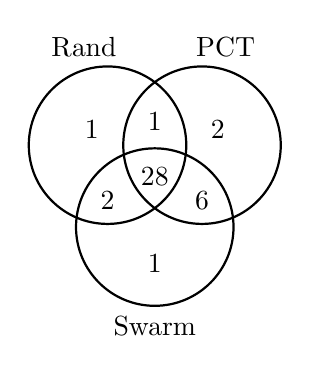
\begin{tikzpicture}[thick]
      \draw (0,0)      circle (1) node[above,shift={(-0.3,1)}] {Rand};
      \draw (1.2,0)    circle (1) node[above,shift={(0.3,1)}]  {PCT};
      \draw (.6,-1.04) circle (1) node[below,shift={(0,-1)}]   {Swarm};

      \node at (.6,-.4)  {28}; % rand  ^ pct   ^ swarm
      \node at (1.2,-.7) {6};  % pct   ^ swarm - rand
      \node at (.6,.3)   {1};  % pct   ^ rand  - swarm
      \node at (0,-.7)   {2};  % rand  ^ swarm - pct
      \node at (1.4,.2)  {2};  % pct   - rand  - swam
      \node at (-.2,.2)  {1};  % rand  - pct   - swarm
      \node at (.6,-1.5) {1};  % swarm - pct   - rand
    \end{tikzpicture}
    \caption{Basic algorithms}\label{fig:bugs-base}
  \end{subfigure}
  \begin{subfigure}{0.3\textwidth}
    \centering
    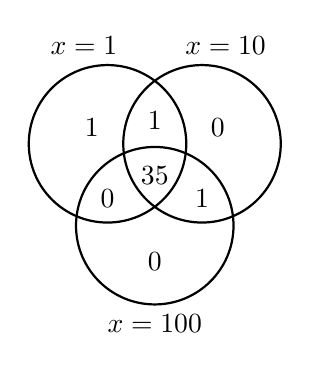
\begin{tikzpicture}[thick]
      \draw (0,0)      circle (1) node[above,shift={(-0.3,1)}] {$x=1$};
      \draw (1.2,0)    circle (1) node[above,shift={(0.3,1)}]  {$x=10$};
      \draw (.6,-1.04) circle (1) node[below,shift={(0,-1)}]   {$x=100$};

      \node at (.6,-.4)  {35}; % 1   ^ 10  ^ 100
      \node at (0,-.7)   {0};  % 1   ^ 100 - 10
      \node at (.6,.3)   {1};  % 1   ^ 10  - 100
      \node at (1.2,-.7) {1};  % 10  ^ 100 - 1
      \node at (-.2,.2)  {1};  % 1   - 10  - 100
      \node at (1.4,.2)  {0};  % 10  - 1   - 100
      \node at (.6,-1.5) {0};  % 100 - 1   - 10
    \end{tikzpicture}
    \caption{Weight re-use}\label{fig:bugs-swarmx}
  \end{subfigure}
  \begin{subfigure}{0.3\textwidth}
    \centering
    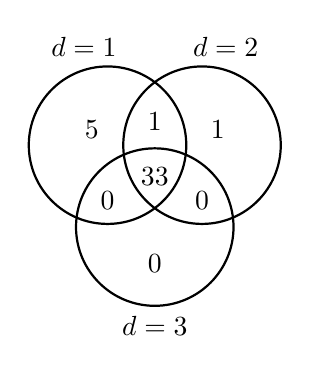
\begin{tikzpicture}[thick]
      \draw (0,0)      circle (1) node[above,shift={(-0.3,1)}] {$d=1$};
      \draw (1.2,0)    circle (1) node[above,shift={(0.3,1)}]  {$d=2$};
      \draw (.6,-1.04) circle (1) node[below,shift={(0,-1)}]   {$d=3$};

      \node at (.6,-.4)  {33}; % 1 ^ 2 ^ 3
      \node at (0,-.7)   {0};  % 1 ^ 3 - 2
      \node at (.6,.3)   {1};  % 1 ^ 2 - 3
      \node at (1.2,-.7) {0};  % 2 ^ 3 - 1
      \node at (-.2,.2)  {5};  % 1 - 2 - 3
      \node at (1.4,.2)  {1};  % 2 - 1 - 3
      \node at (.6,-1.5) {0};  % 3 - 1 - 2
    \end{tikzpicture}
    \caption{Weight changes}\label{fig:bugs-swarmd}
  \end{subfigure}

  \caption{Overlap of bugs found by each scheduling algorithm.}\label{fig:bugs}
\end{figure}

\subsection{Experimental Results}
\label{sec:algorithms-eval-results}

We conducted our experiments in an Ubuntu 12.04 virtual machine, using a
modified version of Maple based on the last commit from 2012\footnote{The same
environment as~\cite{thomson2016}, available
at \url{https://github.com/mc-imperial/sctbench}}.  Other than the
implementation of swarm scheduling, available in \appref{swarm}, the code is
unchanged.

The Venn diagrams in \figref{bugs} show the relative bug-finding ability of each
algorithm.  \figref{bugs-base} summarises the bugs found by controlled random
scheduling, PCT $d=3$, and swarm scheduling $(d,x)=(0,1)$ (which we now call
``Swarm'' for brevity); showing that swarm scheduling performs comparably with
PCT.  Figures~\ref{fig:bugs-swarmx} and~\ref{fig:bugs-swarmd} show the effect of
re-using the swarm weights and of introducing weight change points, we omit
$x=1000$ because it performed worse than the other cases; we see that these
variations have little effect.

\begin{figure}
  \centering
  \input{gen/bugs.tex}
  \caption[Plot of bugs found by each scheduling algorithm.]{The number of bugs found by each algorithm across all benchmarks.  This plot is intended to be viewed with colour.}\label{fig:totalbugs}
\end{figure}

As the techniques we have considered are nondeterministic, it is interesting to
consider their average-case behaviour.  \figref{totalbugs} shows the aggregate
behaviour of the algorithms across all benchmarks as the number of executions
increases; we can see that Swarm initially outperforms PCT, but PCT catches up
as the number of executions increases.  This observation is consistent
with~\cite{thomson2016}.  The plots in \figref{freqbugs} show the average number
of executions to find a bug across all benchmarks; as expected, we can see that
the average number of executions to find \emph{any} bug rapidly converges,
however the average number of schedules to find a \emph{unique} bug does not.
This is due to two factors: (1) the number of bugs is finite; and (2) some bugs
may be out of reach of a particular algorithm.  \tblref{freqs} shows the final
values.  We can see that PCT and Swarm are almost identical, and both
significantly improve upon random scheduling when it comes to
finding \emph{unique} bugs.

\begin{figure}
  \centering
  \begin{subfigure}{0.49\textwidth}
    \centering
    \resizebox{\textwidth}{!}{\input{gen/freqs-total.tex}}
    \caption{All buggy executions.}\label{fig:freqbugs-total}
  \end{subfigure}
  \begin{subfigure}{0.49\textwidth}
    \centering
    \resizebox{\textwidth}{!}{\input{gen/freqs-unique.tex}}
    \caption{Unique buggy executions.}\label{fig:freqbugs-unique}
  \end{subfigure}
  \caption[Plot of average number of executions needed to expose a bug.]{The average number of executions to expose a bug across all benchmarks.  These plots are intended to be viewed with colour.}\label{fig:freqbugs}
\end{figure}

\begin{table}
  \centering
  \begin{tabular}{lrr} \toprule
    Algorithm & Any Bug & A Unique Bug \\ \midrule
    Rand. & 0.071 & 312.5 \\
    PCT   & 0.077 & 270.3 \\
    Swarm & 0.078 & 270.3 \\ \bottomrule
  \end{tabular}
  \caption{Average number of executions needed to find a bug.}\label{tbl:freqs}
\end{table}

Although it is disappointing that Swarm does not improve upon PCT, that it is
able to perform comparably without needing the programmer to first determine the
maximum length of an execution (as is unavoidable in PCT) is encouraging.
